\documentclass[xcolor=table,dvipsnames,svgnames]{beamer}
% Author: alick<alick9188@gmail.com>
% Author: justin <justin.w.xd@gmail.com>

% This file is modified from a solution template for:

% - Giving a talk on some subject.
% - The talk is between 15min and 45min long.
% - Style is ornate.

% Copyright 2004 by Till Tantau <tantau@users.sourceforge.net>.
%
% In principle, this file can be redistributed and/or modified under
% the terms of the GNU Public License, version 2.
%
% However, this file is supposed to be a template to be modified
% for your own needs. For this reason, if you use this file as a
% template and not specifically distribute it as part of a another
% package/program, I grant the extra permission to freely copy and
% modify this file as you see fit and even to delete this copyright
% notice.

\usepackage{tikz}
\mode<presentation>
{
  \usetheme[secheader]{Boadilla}
  \usefonttheme[onlymath]{serif}
  \setbeamercovered{transparent=5}
  \definecolor{thupurple}{HTML}{93278F}
  \definecolor{thudarkpurple}{HTML}{5C307D}
  \definecolor{thulightpurple}{HTML}{BC9BCC}
  \setbeamercolor*{structure}{fg=thupurple}
  \setbeamercolor*{palette primary}{fg=black,bg=thulightpurple}
  \setbeamercolor*{palette secondary}{fg=white,bg=thupurple}
  \setbeamercolor*{palette tertiary}{fg=white,bg=thudarkpurple}
  \setbeamercolor*{palette quaternary}{fg=white,bg=black}
  \setbeamertemplate{itemize item}{\raise1.25pt\hbox{\tikz\draw[fill=fg] (0,0) circle (.3ex);}}
  \setbeamertemplate{itemize subitem}{\color{fg}\tiny\raise1.25pt\hbox{\donotcoloroutermaths$\blacktriangleright$}}
  \setbeamertemplate{itemize subsubitem}{\raise2.5pt\hbox{\tikz\draw[fill=fg] (0,0) rectangle (.7ex, .2ex);}}

  \setbeamertemplate{section in toc}
  {
    \leavevmode\leftskip=2ex%
    \llap{%
      \usebeamerfont*{section number projected}%
      \usebeamercolor{section number projected}%
      \begin{pgfpicture}{0ex}{0ex}{1ex}{2ex}
        \color{bg}
        \pgfpathcircle{\pgfpoint{0pt}{1.2ex}}{1.5ex}
        \pgfusepath{fill}
        \pgftext[at={\pgfpoint{0}{4pt}}]{\color{fg}\fontsize{8}{8}\selectfont\inserttocsectionnumber}
      \end{pgfpicture}\kern1.5ex%
    }%
    \inserttocsection\par
  }
  
  \setbeamertemplate{subsection in toc}
  {
    \leavevmode\leftskip=2.1em%
    \llap{%
      \usebeamerfont*{subsection number projected}%
      \usebeamercolor{subsection number projected}%
      {\color{bg}\tiny\raise1.25pt\hbox{\donotcoloroutermaths$\blacktriangleright$}}
    }%
    \inserttocsubsection\par
  }

  \setlength\leftmargini{1.4em}
  \setlength\leftmarginii{1.4em}
  \setlength\leftmarginiii{1.4em}

}

\usepackage{mflogo} % for \MF, \MP
\usepackage{graphicx}
\graphicspath{{fig/}}
\usepackage{minted}
\usepackage{xspace}
\usepackage{amsmath}
\usepackage{calligra}
\usepackage{cclicenses} % CC symbols
\usepackage{fontspec}
\usepackage[UTF8,nofonts]{ctex}
\usepackage{hologo}
\usepackage{colortbl}
\usepackage{pstricks}
\usepackage{pst-node}
\usepackage{hyperxmp}
\usepackage{booktabs}
\usepackage[normalem]{ulem}
\hypersetup{
pdfauthor={Justin Wong, Alick Zhao},
pdfcopyright={Copyright (C) 2015 by Alick Zhao.
Licensed under CC-BY-SA 4.0. Some rights reserved.},
pdflicenseurl={http://creativecommons.org/licenses/by-sa/4.0/},
}

% From thuthesis user guide
\makeatletter
\def\psRotation#1(#2,#3)#4{%
  \rput{#1}(#2,#3){%
    \psellipticarc[linewidth=.4pt]{->}(0,-0.1)(0.6,0.15){120}{70}
    \ifdim#1pt>\z@\rput[l]{*0}(0.675,0){#4}\else\rput[l](0.675,0){#4}\fi
  }%
}
\makeatother

% For tipa to work.
\newfontfamily\useTIPAfont{Times New Roman}

% xeCJK conf setup
\punctstyle{kaiming}
\renewcommand\CJKfamilydefault{\CJKsfdefault} % for slides

\setCJKmainfont[BoldFont={SimHei},
ItalicFont={KaiTi}]{SimSun}
\setCJKsansfont{WenQuanYi Micro Hei}
\setCJKmonofont{WenQuanYi Micro Hei Mono}

\setCJKfamilyfont{zhsong}{SimSun}
\setCJKfamilyfont{zhhei}{SimHei}
\setCJKfamilyfont{zhkai}{KaiTi}

\newcommand*{\songti}{\CJKfamily{zhsong}} % 宋体
\newcommand*{\heiti}{\CJKfamily{zhhei}}   % 黑体
\newcommand*{\kaishu}{\CJKfamily{zhkai}}  % 楷书

\newcommand{\BibTeX}{\hologo{BibTeX}}
\newcommand{\XeTeX}{\hologo{XeTeX}}
\newcommand{\pdfTeX}{\hologo{pdfTeX}}
\newcommand{\beamer}{\textsc{beamer}}
\def\TeXLive{\TeX{} Live\xspace}
\let\TL=\TeXLive
\newcommand{\ThuThesis}{\textsc{ThuThesis}\xspace}

% From thuthesis user guide.
\def\cmd#1{\texttt{\color{DarkBlue}\footnotesize $\backslash$#1}}
\def\env#1{\texttt{\color{DarkBlue}\footnotesize #1}}
\def\cmdxmp#1#2#3{\small{\texttt{\color{DarkBlue}$\backslash$#1}\{#2\}\hspace{1em}\\ $\Rightarrow$\hspace{1em} {#3}\par\vskip1em}}

% For debugging.
%\includeonlyframes{current}

\title
{如何使用 \LaTeX 排版论文}

\author[汪彧之] % (optional, use only with lots of authors)
{汪彧之\\ \texttt{justin.w.xd@gmail.com}}

\institute[TUNA] % (optional, but mostly needed)
{
  
\includegraphics[height=.2\textheight]{tuna.pdf}
}
% - Use the \inst command only if there are several affiliations.
% - Keep it simple, no one is interested in your street address.

\date[图书馆专题培训讲座] % (optional)
{2015 年 11 月 23 日}

\subject{LaTeX, paper, ThuThesis}

% Delete this, if you do not want the table of contents to pop up at
% the beginning of each subsection:
\AtBeginSubsection[]
{
  \begin{frame}<beamer>{目录}
    \tableofcontents[currentsection,currentsubsection]
  \end{frame}
}


% If you wish to uncover everything in a step-wise fashion, uncomment
% the following command:

%\beamerdefaultoverlayspecification{<+->}

\hypersetup{
%pdfpagemode=FullScreen,
}

\logo{
\includegraphics[height=.15\textheight]{libicon.jpg}}

% \includeonly{introduction}

\begin{document}

\begin{frame}
  \titlepage
\end{frame}

\begin{frame}{目录}
  \tableofcontents
  % You might wish to add the option [pausesections]
\end{frame}


% Since this a solution template for a generic talk, very little can
% be said about how it should be structured. However, the talk length
% of between 15min and 45min and the theme suggest that you stick to
% the following rules:

% - Exactly two or three sections (other than the summary).
% - At *most* three subsections per section.
% - Talk about 30s to 2min per frame. So there should be between about
%   15 and 30 frames, all told.

\section{简介}

\subsection{\TeX 与 \LaTeX}

\begin{frame}[fragile]{\TeX 与 \LaTeX}
  % TODO: photo of Knuth & Lamport
  \begin{columns}[T]
    \column{.8\textwidth}
    \begin{itemize}
      \item \TeX: $\tau\varepsilon\chi$ (\textipa{/'tEx/},
        \textipa{/'tEk/})
        \begin{itemize}
          \item 生成精美图书的排版系统
          \item 最初由 高德纳 (Donald E.~Knuth) 于 1978 年开发
          \item 发音接近``泰赫'',而非``泰克斯'',
            Knuth 对此有\stackon[1pt]{强}{\tiny qi{\v a}ng}迫症
          \item 最新版本为 \TeX\ 3.14159265
          \item 漂亮、美观、稳定、通用
          \item 尤其擅长数学公式排版
        \end{itemize}
      \item \LaTeX\ (\textipa{/'la:tEx/}, \textipa{/'leItEk/})
        \begin{itemize}
          \item Leslie Lamport 开发
          \item 在 \TeX 的基础上的宏包, 降低使用门槛
          \item 极其丰富的宏包,提供扩展功能
          \item 广泛用于学术界,期刊会议论文模板
          \item 大学学位论文模板,如 \ThuThesis
        \end{itemize}
    \end{itemize}
    \column{.2\textwidth}
    %\vspace*{5mm}
    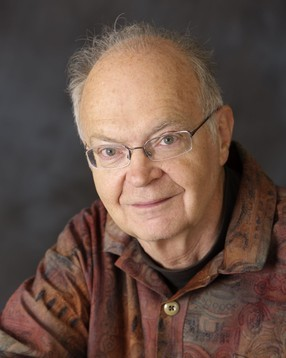
\includegraphics[width=\textwidth]{Knuth.jpg}

    %\vspace*{5mm}
    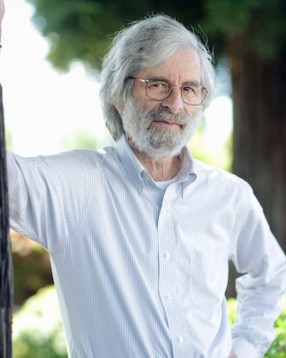
\includegraphics[width=\textwidth]{Lamport.jpg}

  \end{columns}
\end{frame}

\begin{frame}{和 Word 对比}
  \begin{table}[h]
    \centering
    \rowcolors[]{1}{primaryL}{primaryL!40}
    \begin{tabular}{c|c}
      Microsoft\textsuperscript{\textregistered}  Word & \LaTeX \\
      \hline
      字处理工具 & 专业排版软件 \\
      容易上手,简单直观 & 容易上手 \\
      所见即所得 & 所见即所想,所想即所得 \\
      高级功能不易掌握 & 进阶难,但一般用不到 \\
      处理长文档需要丰富经验 & 和短文档处理基本无异 \\
      花费大量时间调格式 & 无需担心格式,专心作者内容 \\
      公式排版差强人意 & 尤其擅长公式排版 \\
      二进制格式,兼容性差 & 文本文件,易读、稳定 \\
      付费商业许可 & 自由免费使用 \\
    \end{tabular}
  \end{table}
\end{frame}

\begin{frame}{\TeX{}排版举例:公式}
  \begin{exampleblock}{无编号公式}
    \begin{equation*}
      \mathcal{F}(\xi)=\int_{-\infty}^{\infty}\!\!
      f(x)\mathrm{e}^{-\mathrm{j}2\pi \xi x}\,\mathrm{d}x
    \end{equation*}
  \end{exampleblock}
  \begin{exampleblock}{多行多列公式}
    % Taken from Mathmode.tex
    \begin{align}
      y & =d & z & =1\\
      y & =cx+d & z & =x+1\\
      y_{12} & =bx^{2}+cx+d & z & =x^{2}+x+1\nonumber \\
      y(x) & =ax^{3}+bx^{2}+cx+d & z & =x^{3}+x^{2}+x+1
    \end{align}
  \end{exampleblock}
\end{frame}

\begin{frame}{\TeX{}排版举例:公式}
  \begin{exampleblock}{编号多行公式}
    % Taken from Mathmode.tex
    \begin{multline}
    A=\lim_{n\rightarrow\infty}\Delta x\left(a^{2}+\left(a^{2}+2a\Delta x+\left(\Delta x\right)^{2}\right)\right.\label{eq:reset}\\
    +\left(a^{2}+2\cdot2a\Delta x+2^{2}\left(\Delta x\right)^{2}\right)\\
    +\left(a^{2}+2\cdot3a\Delta x+3^{2}\left(\Delta x\right)^{2}\right)\\
    +\ldots\\
    \left.+\left(a^{2}+2\cdot(n-1)a\Delta x+(n-1)^{2}\left(\Delta x\right)^{2}\right)\right)\\
    =\frac{1}{3}\left(b^{3}-a^{3}\right)
  \end{multline}
\end{exampleblock}
\end{frame}

\begin{frame}{\TeX{}排版举例:图形}
  % From thuthesis user guide.
  \begin{minipage}[c]{0.3\linewidth}
    \psset{unit=0.8cm}
    \begin{pspicture}(-1.75,-3)(3.25,4)
      \psline[linewidth=0.25pt](0,0)(0,4)
      \rput[tl]{0}(0.2,2){$\vec e_z$}
      \rput[tr]{0}(-0.9,1.4){$\vec e$}
      \rput[tl]{0}(2.8,-1.1){$\vec C_{ptm{ext}}$}
      \rput[br]{0}(-0.3,2.1){$\theta$}
      \rput{25}(0,0){%
      \psframe[fillstyle=solid,fillcolor=lightgray,linewidth=.8pt](-0.1,-3.2)(0.1,0)}
      \rput{25}(0,0){%
      \psellipse[fillstyle=solid,fillcolor=yellow,linewidth=3pt](0,0)(1.5,0.5)}
      \rput{25}(0,0){%
      \psframe[fillstyle=solid,fillcolor=lightgray,linewidth=.8pt](-0.1,0)(0.1,3.2)}
      \rput{25}(0,0){\psline[linecolor=red,linewidth=1.5pt]{->}(0,0)(0.,2)}
      \psRotation{0}(0,3.5){$\dot\phi$}
      \psRotation{25}(-1.2,2.6){$\dot\psi$}
      \psline[linecolor=red,linewidth=1.25pt]{->}(0,0)(0,2)
      \psline[linecolor=red,linewidth=1.25pt]{->}(0,0)(3,-1)
      \psline[linecolor=red,linewidth=1.25pt]{->}(0,0)(2.85,-0.95)
      \psarc{->}{2.1}{90}{112.5}
      \rput[bl](.1,.01){C}
    \end{pspicture}
  \end{minipage}\hspace{1cm}
  \begin{minipage}[t]{0.5\linewidth}
    \psset{unit=0.3cm}
    \begin{pspicture}(1,2)(18,14)
      %\psgrid[gridcolor=lightgray,subgriddiv=0,subgridcolor=lightgray]
      %
      \psline[linewidth=1pt,linecolor=black](6,0.5)(6,14)
      \psline[linewidth=1pt,linecolor=black](1,8.5)(6,7)
      \psline[linewidth=1pt,linecolor=black](1.5,5.5)(11,8.5)
      %
      \rput(17,3){$x$}
      \rput(5.5,13){$y$}
      \rput(10.5,8.75){$z$}
      \rput(11,7.1){$\vec{r}$}
      %
      \psline[linewidth=1.5pt,linecolor=black]{<->}(6,7)(6,11.25)
      \rput(5.35,9.4){$R$}
      \psline[linewidth=1.5pt,linecolor=Green]{->}(6.5,12)(4.75,12)
      \rput(7.5,12.8){ $I d\vec{l}$}
      %
      \psellipse[doubleline=true,doublecolor=yellow,doublesep=3pt,linecolor=blue](6,7)(3,4.5)
      \psline[linewidth=1pt,linecolor=black](6,7)(17.5,3.5)
      \psline[linewidth=1.5pt,linecolor=black]{->}(6,11.38)(11.95,5.225)
      %
      \psarc[linewidth=1.5pt,linecolor=gray](6,8){3.4}{85}{95}
      %
      \psline[linewidth=1.5pt,linecolor=gray]{->}(12,5.15)(12,8.15)
      \psline[linewidth=1.5pt,linecolor=black]{->}(12,5.15)(15,7.25)
      \psline[linewidth=1.5pt,linecolor=gray]{->}(12,5.15)(15,4.25)
      %
      \psline[linewidth=1pt,linecolor=black](12,8.15)(15,7.25)(15,4.25)
      %
      \Cnode*[linecolor=black,radius=0.1cm](12,5.15){a}
      \rput(11.5,4.5){ $P$}
      %
      \rput(12.5,8.9){$dB_y$}
      \rput(14.5,3.4){$dB_x$}
      \rput(15.5,8){ $d \boldmath{\vec{B}}$}
      %
      \psarc[linewidth=1pt]{<->}(12,5){5.5}{133}{161}
      \rput(7.2,8.5){ $\theta$}
    \end{pspicture}
    \medskip

    %\hspace{2cm}
    \begin{figure}[h]
      \centering
      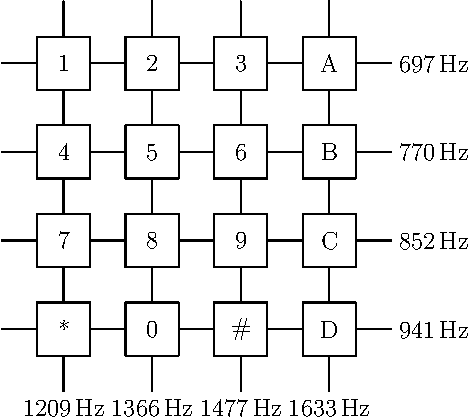
\includegraphics[height=.33\textheight]{dtmf.pdf}
    \end{figure}
  \end{minipage}
\end{frame}

\begin{frame}{\TeX{}排版举例:文档}
  \begin{columns}
    \begin{column}{.45\textwidth}
      \begin{figure}[h]
        \centering
        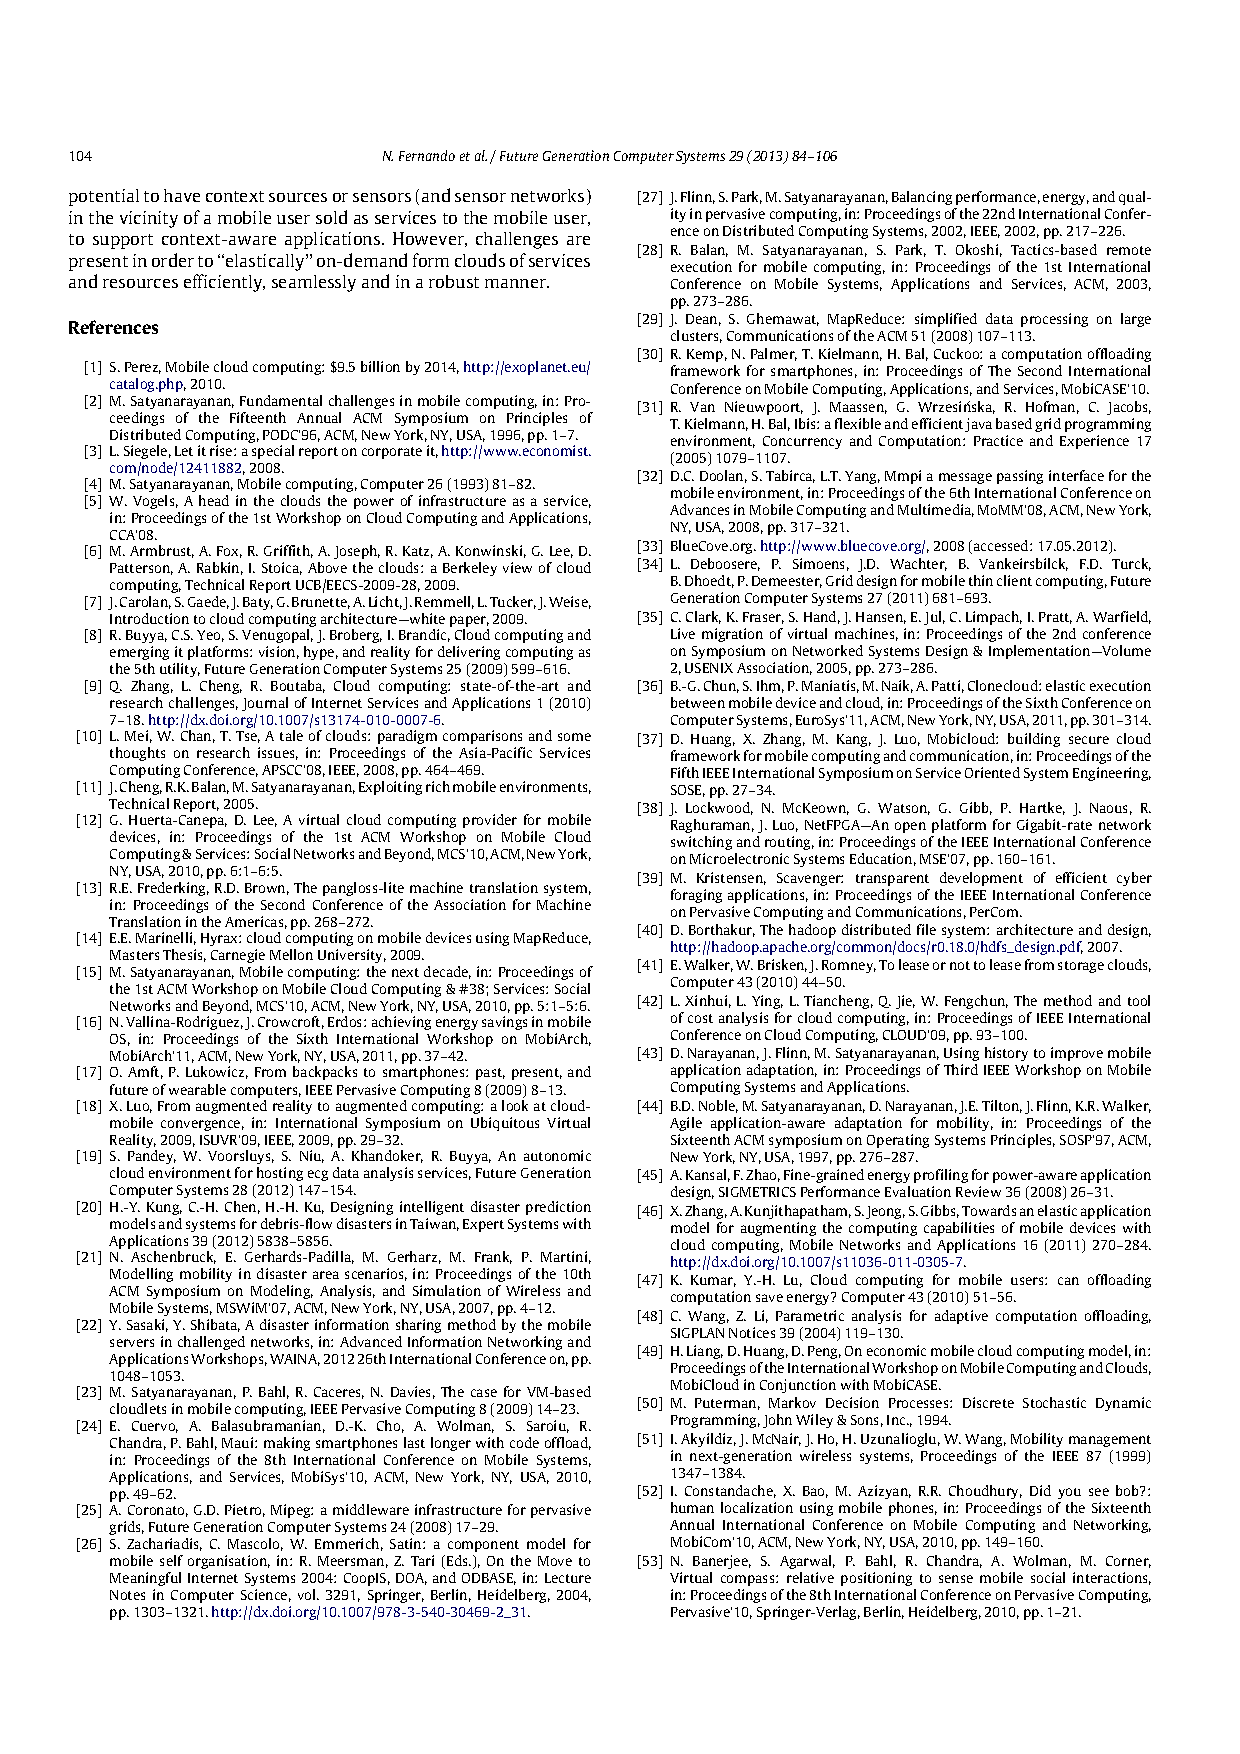
\includegraphics[width=.8\textwidth]{references.pdf}
      \end{figure}
    \end{column}
    \begin{column}{.45\textwidth}
      \begin{figure}[h]
        \centering
        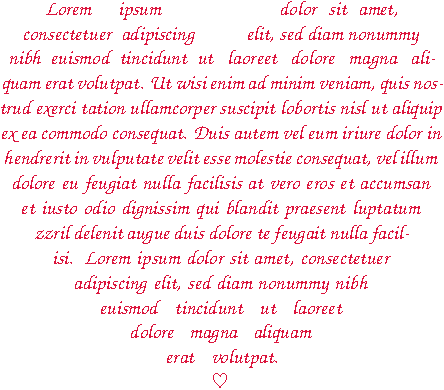
\includegraphics[width=.8\textwidth]{shapepar.pdf}
      \end{figure}
    \end{column}
  \end{columns}
\end{frame}

\begin{frame}{\TeX{}排版举例:幻灯片}
  \begin{columns}
    \begin{column}{.45\textwidth}
      \begin{figure}[h]
        \centering
        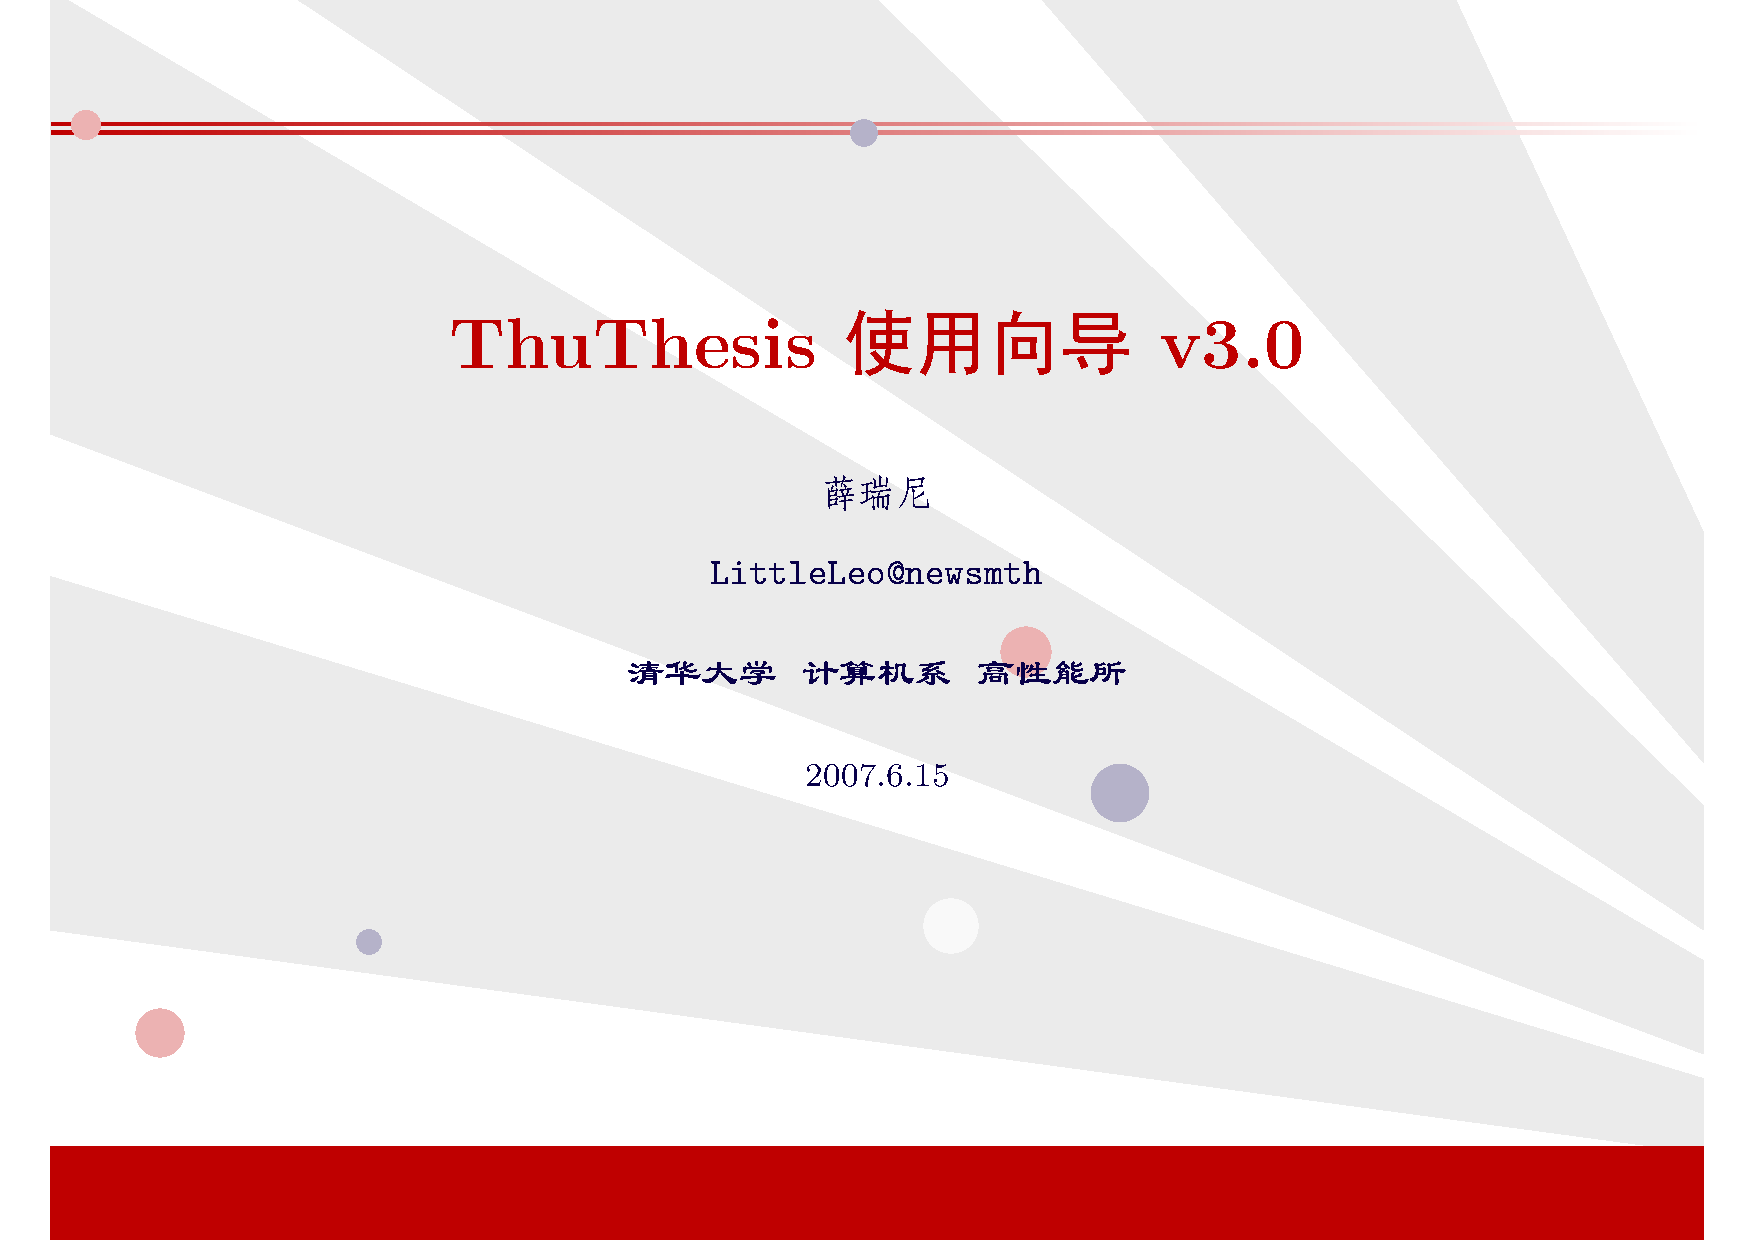
\includegraphics[width=\textwidth]{slides-powerdot.pdf}
      \end{figure}
    \end{column}
    \begin{column}{.45\textwidth}
      \begin{figure}[h]
        \centering
        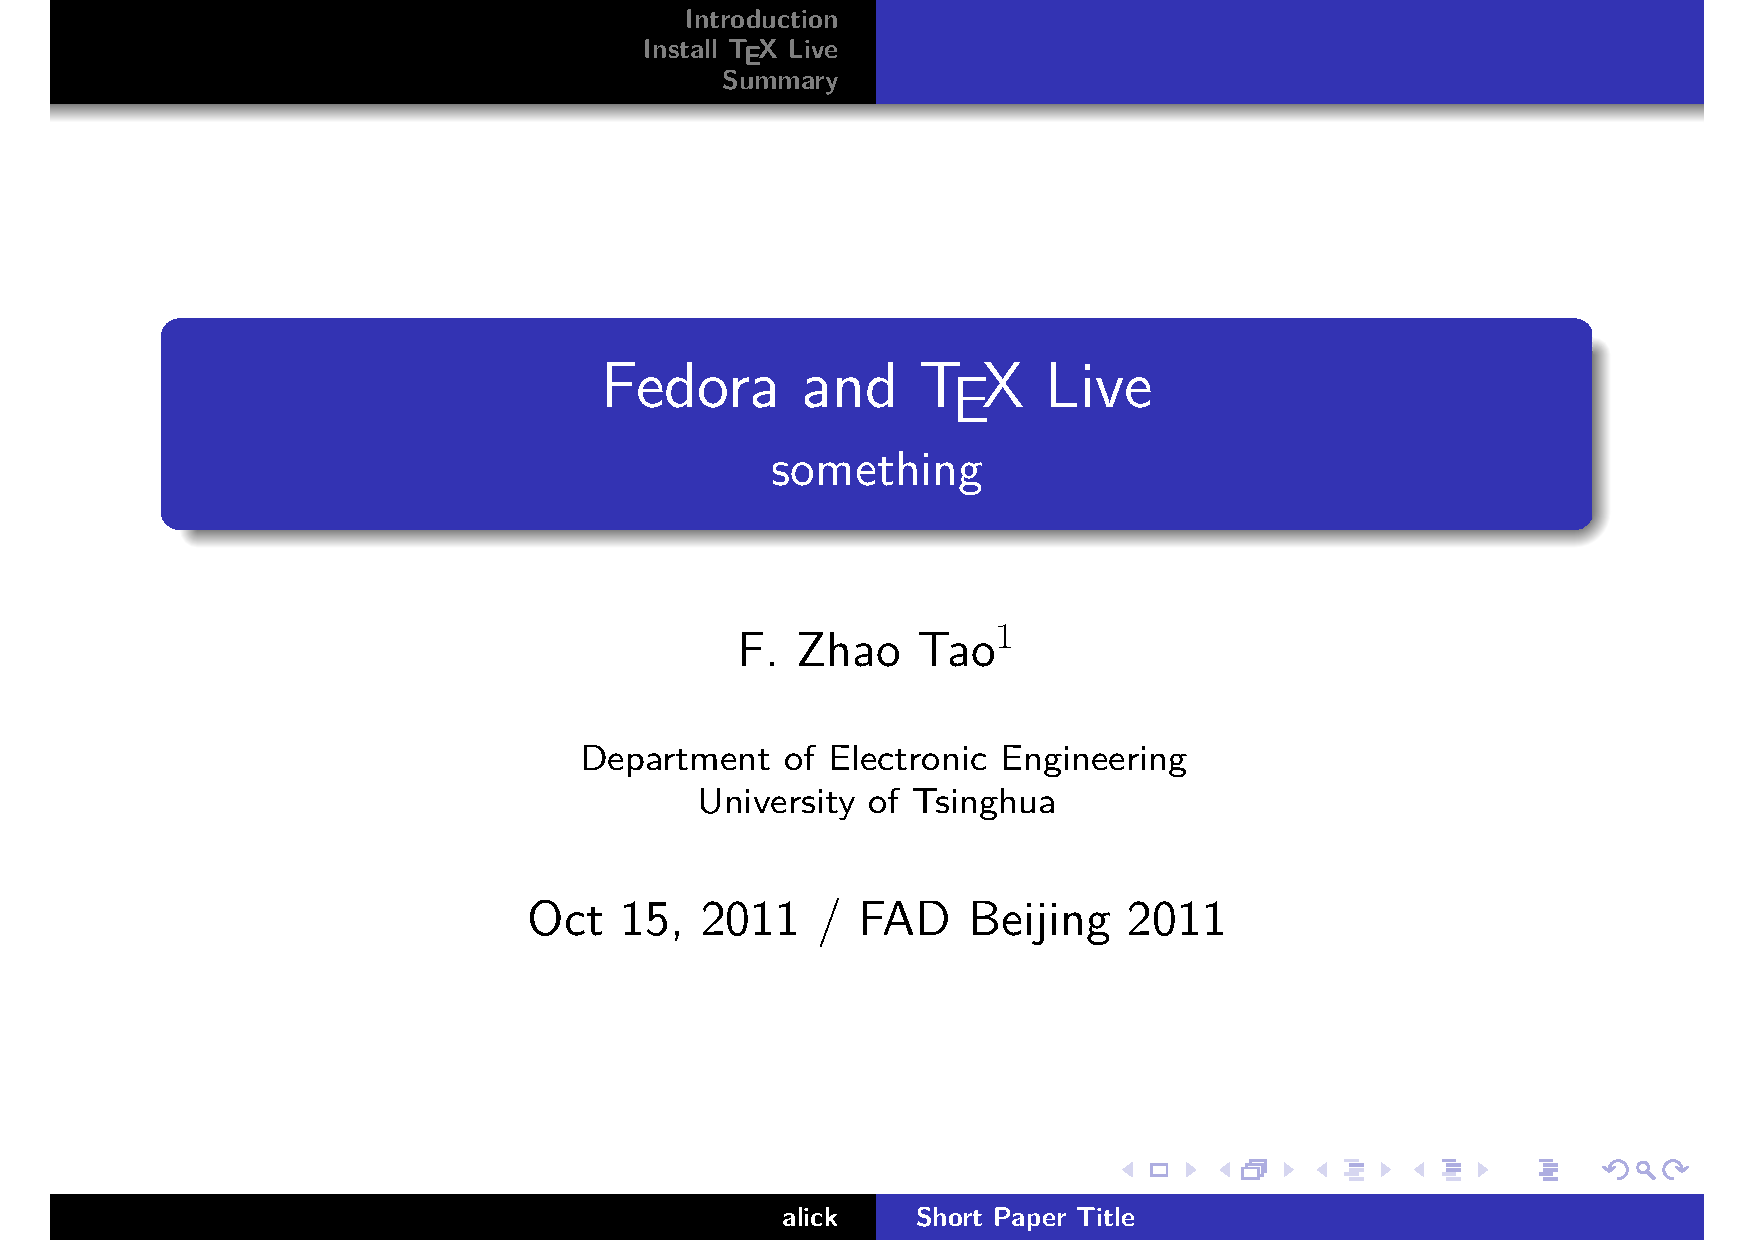
\includegraphics[width=\textwidth]{slides-beamer.pdf}
      \end{figure}
    \end{column}
  \end{columns}
\end{frame}

\subsection{安装}

\begin{frame}{如何安装 \hologo{(La)TeX}?}
  \begin{itemize}
    \item \TeX{}发行版(Distro)
      \begin{itemize}
        \item \TeX{}实用工具大集合:引擎、宏包、文档等
        \item 常见\TeX{}发行版:
          \alert{\TL}, \CTeX, \MiKTeX, \MacTeX
      \end{itemize}
    \item \TL
      \begin{itemize}
        \item 跨平台:Windows, Linux, Mac OS X (\MacTeX)
        \item 每年一个新版本发布,当前 \TL 2017(已经冻结,2018 即将发布)
      \end{itemize}
    \item \MiKTeX
      \begin{itemize}
        \item 专为 Windows 开发
        \item 个人维护,作者失联,新版跳票
      \end{itemize}
    \item \CTeX
      \begin{itemize}
        \item 中科院吴凌云研究员基于 \MiKTeX 开发
        \item 极大的方便了中文 \TeX 用户
        \item 2012 之后停止开发,不建议再使用
      \end{itemize}
  \end{itemize}
\end{frame}

\begin{frame}[fragile]
  \frametitle{下载}
  \begin{itemize}
    \item 注意!
      \begin{itemize}
        \item 不能放在带有中文的路径中
      \end{itemize}
    \item 离线安装镜像 (约3GB大小)
      \begin{itemize}
        \item {\footnotesize
          \url{https://mirrors.tuna.tsinghua.edu.cn/CTAN/systems/texlive/Images/texlive.iso}}
      \end{itemize}
    \item 在线安装包 (和相应的校验文件,以 .sha256 结尾)
      \begin{itemize} % several mirror url
        \item {\footnotesize
          \url{https://mirrors.tuna.tsinghua.edu.cn/CTAN/systems/texlive/tlnet/}
        }
        \item 更多可见 \url{http://mirror.ctan.org/README.mirrors}
      \end{itemize}

    \item 可选步骤:校验安装包
      \begin{lstlisting}[language=tex]
LANG=C sha256sum --check install-tl-unx.tar.gz.sha256
install-tl-unx.tar.gz: OK
      \end{lstlisting}

  \end{itemize}
\end{frame}

\begin{frame}[fragile]
  \frametitle{下载}
  \begin{itemize}
    \item Windows
      \begin{itemize}
        \item 双击下载的安装程序
        \item 切换默认仓库为国内镜像:加速网络下载
      \end{itemize}
    \item Mac OS X
      \begin{itemize}
        \item \texttt{https://mirrors.tuna.tsinghua.edu.cn/\\CTAN/systems/mac/mactex/MacTeX.pkg}
      \end{itemize}
    \item Linux
      \begin{itemize}
        \item 图形安装界面需要 Perl Tk 模块:
          \begin{lstlisting}
yum install perl-Tk 或 apt-get install perl-tk
sudo mkdir /usr/local/texlive
sudo chown yourname:yourname /usr/local/texlive
./install-tl -gui -repository \
  https://mirrors.tuna.tsinghua.edu.cn/CTAN/systems/texlive/tlnet/
        \end{lstlisting}
      \end{itemize}
\item 截图\dots
\end{itemize}
\end{frame}

\begin{frame}
  \begin{figure}[h]
    \centering
    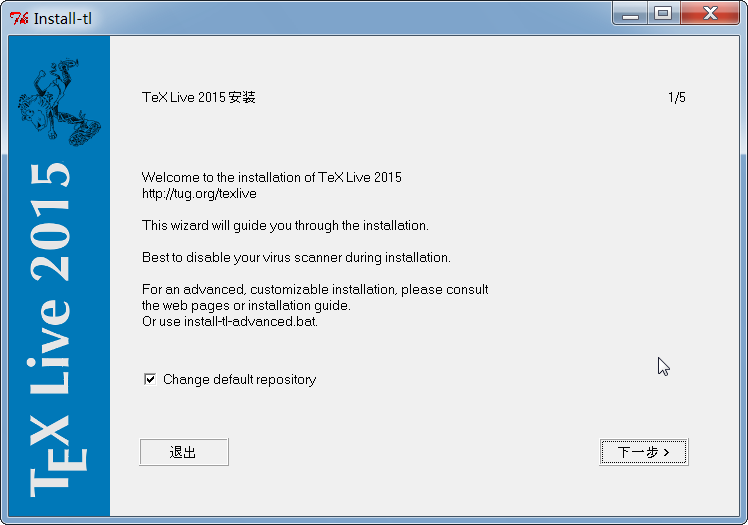
\includegraphics[scale=0.7]{install-tl-0.png}
  \end{figure}
\end{frame}

\begin{frame}
  \begin{figure}[h]
    \centering
    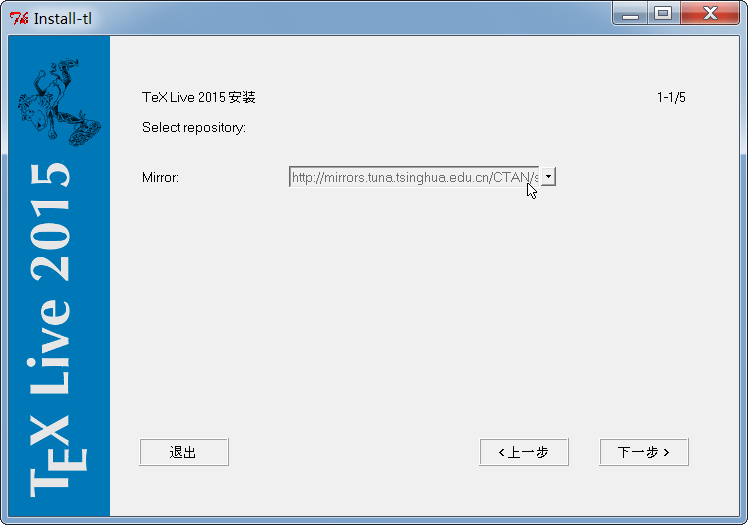
\includegraphics[scale=0.7]{install-tl-1.png}
  \end{figure}
\end{frame}

\begin{frame}
  \begin{figure}[h]
    \centering
    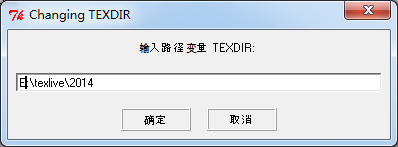
\includegraphics[height=.25\textheight]{simple3-dir.png}\\
    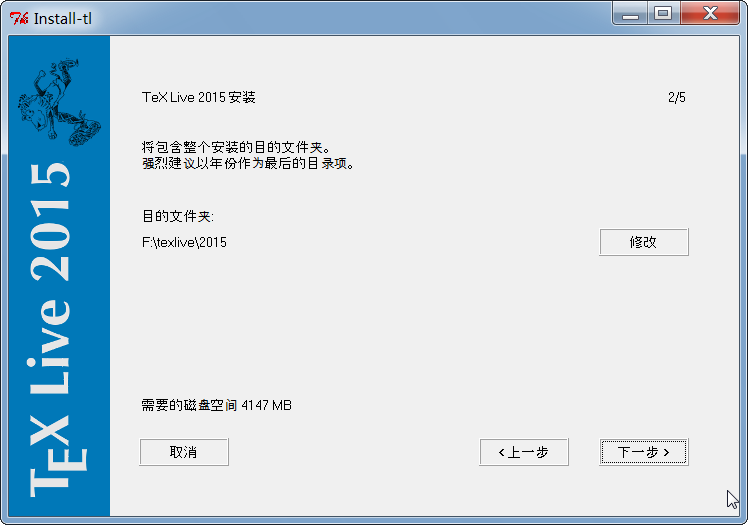
\includegraphics[scale=0.5]{install-tl-2.png}
  \end{figure}
\end{frame}

\begin{frame}
  \begin{figure}[h]
    \centering
    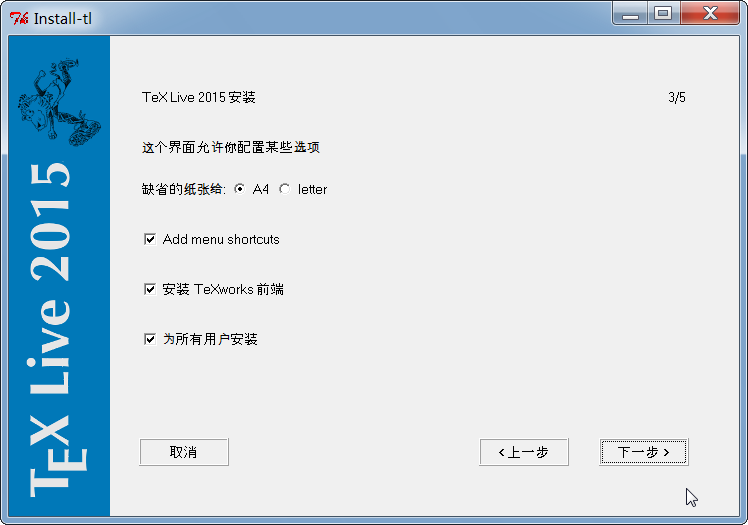
\includegraphics[scale=0.7]{install-tl-3.png}
  \end{figure}
\end{frame}

% 准备安装

\begin{frame}
  \begin{figure}[h]
    \centering
    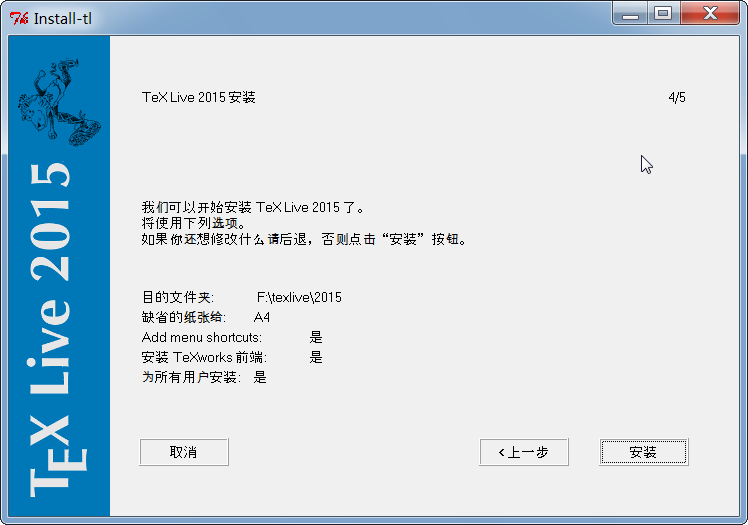
\includegraphics[scale=0.7]{install-tl-4.png}
  \end{figure}
\end{frame}

% 安装进行中
\begin{frame}
  \begin{figure}[h]
    \centering
    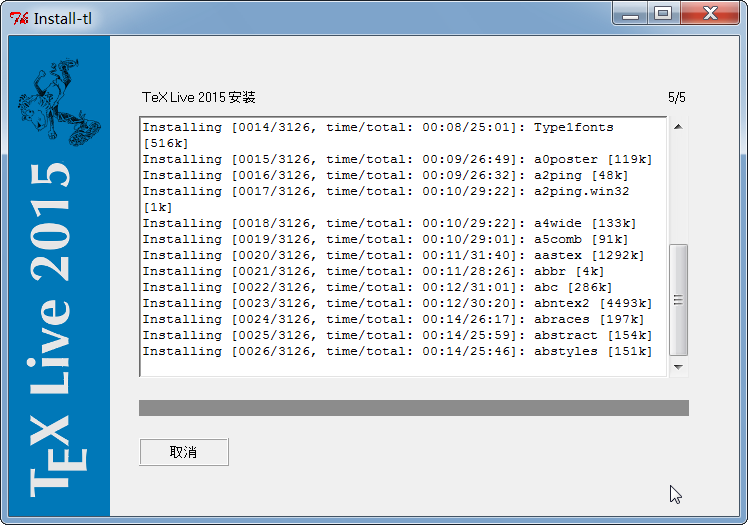
\includegraphics[scale=0.7]{install-tl-5.png}
  \end{figure}
\end{frame}

% 安装后期
\begin{frame}
  \begin{figure}[h]
    \centering
    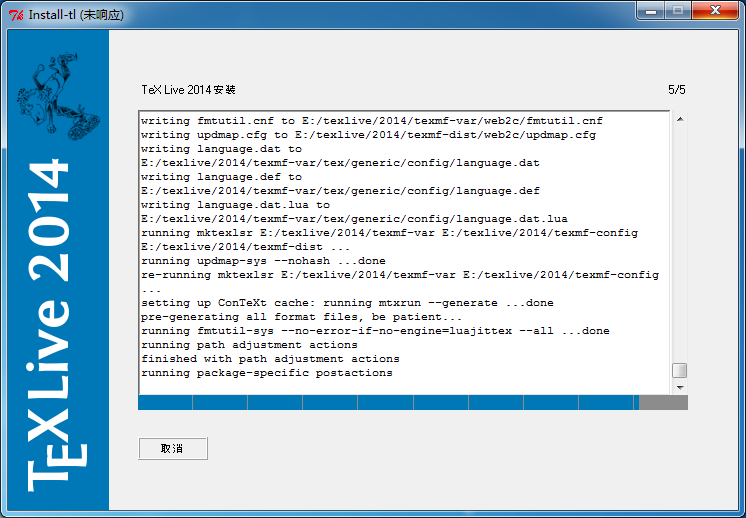
\includegraphics[scale=0.5]{simple8-postinstall.png}
  \end{figure}
\end{frame}

% 安装完成
\begin{frame}
  \begin{figure}[h]
    \centering
    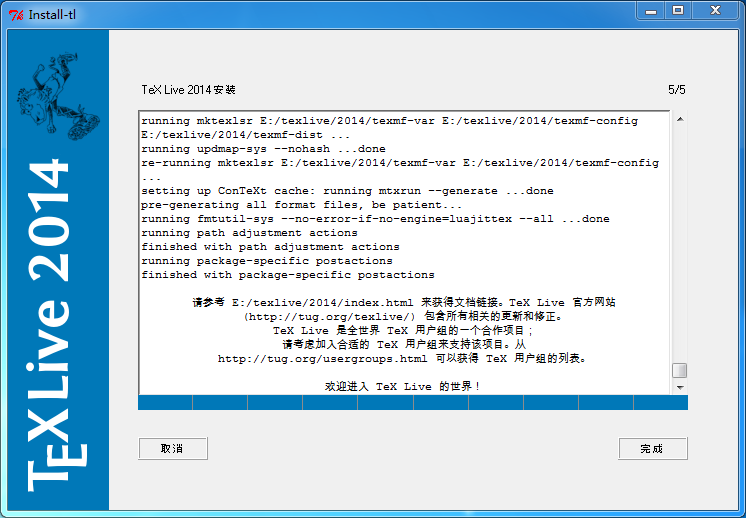
\includegraphics[width=.5\textwidth]{simple9-installed.png}%
    \hspace{2em}
    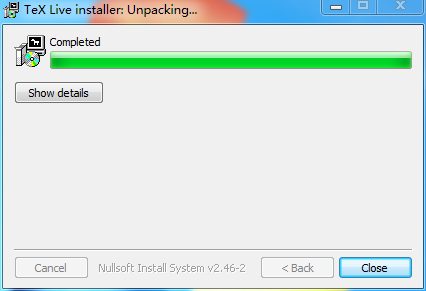
\includegraphics[width=.3\textwidth]{simple10-close.png}
  \end{figure}

  \centering Windows 上安装过程比较慢,尤其是最后的生成索引阶段,请耐心等待

\end{frame}

\begin{frame}[fragile]
  \frametitle{网络安装后配置(仅 Linux)}
  \begin{itemize}
    \item
      添加环境变量到 \nolinkurl{~/.bash_profile} 文件:
      \begin{lstlisting}[language=bash]
export PATH=/usr/local/texlive/2017/bin/x86_64-linux:$PATH
export MANPATH=/usr/local/texlive/2017/texmf/doc/man:$MANPATH
export INFOPATH=/usr/local/texlive/2017/texmf/doc/info:$INFOPATH
      \end{lstlisting}
  \item
    打开 \TeXLive 指南中文版 ``texlive-zh-cn.pdf'',
    关注第 3.4 节
      \begin{lstlisting}[basicstyle=\ttfamily]
texdoc texlive-zh
      \end{lstlisting}
  \end{itemize}
\end{frame}

\begin{frame}[fragile]
  \frametitle{网络安装后配置(仅 Linux)}
  \begin{itemize}
  \item
    \XeTeX\ 系统字体配置
    \begin{lstlisting}[language=bash]
cp /usr/local/texlive/2017/texmf-var/fonts/conf/texlive-fontconfig.conf \
  /etc/fonts/conf.d/09-texlive.conf
fc-cache -fsv
    \end{lstlisting}
  \item 让系统的包管理器知道 TeX Live 已经装过了,所以安装一个 dummy package
    \begin{itemize}
      \item Arch Linux 用户装 AUR 里的 \verb|texlive-dummy|
      \item Debian/Ubuntu 用户参照手册做一个包即可
        \url{https://www.tug.org/texlive/debian.html\#vanilla}
      \item Feodra 用户可以在
        \url{https://copr.fedoraproject.org/coprs/fatka/texlive-dummy/} 下载
    \end{itemize}
  \item 教程可参考: \url{http://zhuanlan.zhihu.com/LaTeX/20069414}
  \end{itemize}
\end{frame}

\begin{frame}{编辑器配置}
  \begin{itemize}
    \item \TeX{}编辑器
      \begin{itemize}
        \item 专用编辑器:TeXworks、\alert{TeXStudio}、TeXmaker、WinEdt 等
        \item 通用编辑器(加 LaTeX 插件):Vim、Emacs、VS Code、Sublime、Atom 等
      \end{itemize}
  \end{itemize}
  \begin{exampleblock}{TeXStudio 配置}
    \begin{itemize}
      \item Options -> Configure TeXstudio
        \begin{itemize}
          \item Build:Default Compiler 选择 XeLaTeX
          \item 搜索框输入 Line Number -> Adv. Editor -> 打开行号
        \end{itemize}
    \end{itemize}
  \end{exampleblock}
\end{frame}


\begin{frame}[fragile]
  \frametitle{使用在线协作平台}
  \begin{itemize}
    \item 通过在线平台编辑、编译
      \begin{itemize}
        \item OverLeaf, ShareLaTeX(公司已经合并,站点独立运作)
      \end{itemize}
    \item 免去安装/升级等一系列烦恼
    \item 可以多人协作
    \item 支持中文,但有时需要自己上传字体
      \begin{itemize}
        \item OverLeaf 可直接使用 ctex 宏集
      \end{itemize}
    \item 容量有一定限制
  \end{itemize}
\end{frame}


\begin{frame}{后期安装宏包}
  \begin{exampleblock}{很多时候需要自己安装宏包}
    \vspace*{-3mm}
    \begin{itemize}
      \item 发行版没有预装
      \item 宏包需要更新
    \end{itemize}
  \end{exampleblock}
  \vspace*{-3mm}
  \begin{exampleblock}{\TL}
    \vspace*{-3mm}
    \begin{itemize}
      \item 开始菜单里找 Tex Live Manager
      \item 设置仓库地址 \texttt{tlmgr option repository} {\footnotesize\ttfamily
        https://mirrors.tuna.tsinghua.edu.cn/CTAN/systems/texlive/tlnet}
      \item 使用 \texttt{tlmgr install <pkgname>}命令
    \end{itemize}
  \end{exampleblock}
  \vspace*{-3mm}
  \begin{exampleblock}{\CTeX 或 \MiKTeX}
    \vspace*{-3mm}
    \begin{itemize}
      \item 开始菜单里找 CTeX / MiKTeX -> Package Manager
      \item 在 WinEdt 里 MiKTex Options -> Packages
    \end{itemize}
  \end{exampleblock}
\end{frame}

%\begin{frame}
%\frametitle{网络安装后测试}
%\framesubtitle{English 测试}

%\begin{exampleblock}{使用已安装的示例文件}
%\begin{itemize}
%\item \texttt{latex sample2e.tex \#} .tex $\rightarrow$ .dvi (device independent)

%\texttt{xdvi sample2e.dvi \#} also try dvipdf sample2e.dvi
%\item try \texttt{pdflatex sample2e} directly
%\item \texttt{xetex opentype-info.tex \#} test of xetex's OpenType support
%\end{itemize}

%\end{exampleblock}
%\end{frame}

\begin{frame}[fragile]
  \frametitle{安装后测试}

  \begin{itemize}
    \item 编辑 \texttt{hello.tex} (Windows 下不要用中文文件名;注意
      \LaTeX{} 文档对大小写敏感。)
      \lstset{language=[LaTeX]TeX}
      \begin{card} \begin{lstlisting}[basicstyle=\ttfamily]
\documentclass{ctexarticle} % 使用 ctex 适配过的 article 文档类
\begin{document}
\TeX{}你好!
\end{document}
        \end{lstlisting}\end{card}
      \begin{itemize}
        \item Windows 下缺省使用中易字体
        \item Linux、Mac OS X 下需要注意字体(参见 ctex 文档)
      \end{itemize}
    \item 使用 XeLaTeX 引擎编译,得到 PDF 文档
      \begin{center}
        \fbox{\textrm \TeX{}\songti 你好!}
      \end{center}
  \end{itemize}
\end{frame}

%%% vim: set ts=2 sts=2 sw=2 isk+=\: et tw=80 cc=+1 formatoptions+=mM:

% !TeX encoding = UTF-8
% !TeX program = latexmk
% !TeX root = latex-talk.tex

\section{学术论文排版}
\subsection{\LaTeX{} 排版入门}

\begin{frame}[fragile]
  \frametitle{引擎与格式}
  \begin{itemize}
    \item \textbf{引擎}:\TeX{} 的实现

      \begin{itemize}
        \item \pdfTeX{}:直接生成 PDF,支持 micro-typography
        \item \XeTeX{}:支持 Unicode、OpenType 与复杂文字编排(CTL)
        \item \LuaTeX{}:支持 Unicode,内联 Lua,支持 OpenType
        \item (u)p\TeX{}:日本方面推动,生成 |.dvi|,(支持 Unicode)
        \item Ap\TeX{}:底层 CJK 支持,内联 Ruby,Color Emoji
      \end{itemize}

    \item \textbf{格式}:\TeX{} 的语言扩展(命令封装)

      \begin{itemize}
        \item plain \TeX{}:Knuth 同志专用
        \item \LaTeX{}:排版科技类文章的事实标准
        \item Con\TeX t:基于 \LuaTeX{} 实现,优雅、易用(吗?)
      \end{itemize}

    \item \textbf{程序}:引擎 + dump 后的格式代码

      \begin{itemize}
        \item \alert{英文文章:\pdfLaTeX{}、\XeLaTeX{} 或 \LuaLaTeX{}}
        \item \alert{中文文章:\XeLaTeX{} 或 \LuaLaTeX{}}
      \end{itemize}
  \end{itemize}
\end{frame}

\begin{frame}[fragile]
  \frametitle{编译}
  \begin{itemize}
    \item 现代 \TeX{} 引擎均可直接生成 PDF
    \item 命令行

      \begin{itemize}
        \item |pdflatex|/|xelatex|/|lualatex| + |<文件名>[.tex]|
        \item 多次编译:每次均需要读取并处理中间文件
        \item 推荐 \pkg{latexmk}:运行 |latexmk [<选项>] <文件名>| 即可自动完成所有工作
      \end{itemize}

    \item 编辑器

      \begin{itemize}
        \item 按钮的背后仍然是命令
        \item |PATH| 环境变量:确定可执行文件的位置
        \item VS Code + \LaTeX{} Workshop:配置 |tools| 和 |recipes|
      \end{itemize}
  \end{itemize}
\end{frame}


\begin{frame}[fragile]{文件结构}
  \lstset{language=[LaTeX]TeX}
  \begin{lstlisting}[basicstyle=\ttfamily]
\documentclass[a4paper]{article}
% 文档类型,如 article,[]内是选项,如 a4paper
% 这里开始是导言区
\usepackage{graphicx} % 引用宏包
\graphicspath{{fig/}} % 设置图片目录
% 导言区到此为止
\begin{document}
这里开始是正文
\end{document}
  \end{lstlisting}
\end{frame}

\begin{frame}[fragile]{\LaTeX{}“命令”}
  \framesubtitle{\emph{宏} (Macro)、或者\emph{控制序列} (control sequence)}
\begin{itemize}
\item 简单命令
  \begin{itemize}
    \item \verb|\命令|\hspace{2em}
    \verb|{\songti 中国人民解放军}| ~$\Rightarrow$ {\songti 中国人民解放军}
  \item \verb|\命令[可选参数]{必选参数}|\\
\verb|\section[精简标题]{这个题目实在太长了放到目录里面不太好看}|\\
$\Rightarrow$ {\heiti 1.1 \hspace{1em} \songti 这个题目实在太长了放到目录里面不太好看}
  \end{itemize}
\item 环境
  \begin{columns}[c]
  \begin{column}{0.45\textwidth}
    \begin{lstlisting}[basicstyle=\ttfamily]
\begin{equation*}
  a^2-b^2=(a+b)(a-b)
\end{equation*}
\end{lstlisting}
\end{column}\hspace{1em}
  \begin{column}{0.45\textwidth}
$ a^2-b^2=(a+b)(a-b)$
\end{column}
  \end{columns}
\end{itemize}
\end{frame}

\begin{frame}[fragile]{\LaTeX{} 常用命令}
  \begin{exampleblock}{简单命令}
\centering
\footnotesize
  \begin{tabular}{llll}
    \cmd{chapter} & \cmd{section} & \cmd{subsection} & \cmd{paragraph} \\
    章 & 节 & 小节 & 带题头段落 \\\hline
    \cmd{centering} & \cmd{emph} & \cmd{verb} & \cmd{url} \\
   居中对齐         &  强调      & 原样输出   & 超链接 \\\hline
  \cmd{footnote} & \cmd{item} & \cmd{caption} & \cmd{includegraphics} \\
   脚注 & 列表条目 & 标题 & 插入图片 \\\hline
  \cmd{label} & \cmd{cite} & \cmd{ref} \\
  标号 & 引用参考文献 & 引用图表公式等\\\hline
  \end{tabular}
\end{exampleblock}
\end{frame}
\begin{frame}[fragile]{\LaTeX{} 常用命令}
\begin{exampleblock}{环境}
\centering
\footnotesize
\begin{tabular}{lll}
  \env{table} & \env{figure} & \env{equation}\\
  表格 & 图片 & 公式 \\\hline
  \env{itemize} & \env{enumerate} & \env{description}\\
  无编号列表 & 编号列表 & 描述 \\\hline
\end{tabular}
\end{exampleblock}
\end{frame}
%
\begin{frame}{\LaTeX{}命令举例}
\cmdxmp{chapter}{前言}{\heiti 第 1 章\hspace{1em} 前言}
\cmdxmp{section[精简标题]}{这个题目实在太长了放到目录里面不太好看}{\heiti 1.1
  \hspace{1em} 这个题目实在太长了放到目录里面不太好看}
\cmdxmp{footnote}{我是可爱的脚注}{前方高能\footnote{我是可爱的脚注}}
\end{frame}

\begin{frame}[fragile]{\LaTeX{} 环境举例}
  \begin{minipage}{0.4\linewidth}
    \begin{lstlisting}[basicstyle=\ttfamily\small]
\begin{itemize}
  \item 一条
  \item 次条
  \item 这一条可以分为 ...
    \begin{itemize}
      \item 子一条
    \end{itemize}
\end{itemize}
\end{lstlisting}
  \end{minipage}\hspace{1.5cm}
  \begin{minipage}{0.4\linewidth}
\begin{itemize}
  \item 一条
  \item 次条
  \item 这一条可以分为 ...
    \begin{itemize}
      \item 子一条
    \end{itemize}
\end{itemize}
  \end{minipage}
\medskip

  \begin{minipage}{0.4\linewidth}
\begin{lstlisting}
\begin{enumerate}
  \item 一条
  \item 次条
  \item 再条
\end{enumerate}
\end{lstlisting}
  \end{minipage}\hspace{1.5cm}
  \begin{minipage}{0.4\linewidth}
\begin{enumerate}
  \item 一条
  \item 次条
  \item 再条
\end{enumerate}
  \end{minipage}
\end{frame}
%

\begin{frame}[fragile]{\LaTeX{} 数学公式}

\begin{columns}
\begin{column}{.5\textwidth}
\begin{lstlisting}[basicstyle=\ttfamily\small]
$V = \frac{4}{3}\pi r^3$

\[
  V = \frac{4}{3}\pi r^3
\]

\begin{equation}
\label{eq:vsphere}
V = \frac{4}{3}\pi r^3
\end{equation}
\end{lstlisting}
\end{column}

\begin{column}{.5\textwidth}
$V = \frac{4}{3}\pi r^3$

\[
  V = \frac{4}{3}\pi r^3
\]

\begin{equation}
\label{eq:vsphere}
V = \frac{4}{3}\pi r^3
\end{equation}
\end{column}
\end{columns}

\end{frame}

\begin{frame}[fragile]{\LaTeX{} 数学公式}
\begin{itemize}
\item 数学公式排版是 \LaTeX{} 的绝对强项
\item 数学排版需要进入数学模式,引用 \texttt{amsmath} 宏包
	\begin{itemize}
	\item 用单个美元符号(\verb|$|) 包围起来的内容是 {\bf 行内公式}
  \item 用两个美元符号(\verb|$$|) (不推荐)或 \verb|\[ \]| 包围起来的是 {\bf 单行公式} 或 {\bf 行间公式}
	\item 使用数学环境,例如 \texttt{equation} 环境内的公式会自动加上编号,
		\texttt{align} 环境用于多行公式(例如方程组、多个并列条件等)
  \end{itemize}
\item 寻找符号
    \begin{itemize}
      \item 运行 \texttt{texdoc symbols} 查看符号表
      \item S. Pakin. \emph{The Comprehensive \LaTeX{} Symbol List}
            \link{https://ctan.org/pkg/comprehensive}
      \item 手写识别(有趣但不全):Detexify \link{http://detexify.kirelabs.org}
    \end{itemize}
\item MathType 也可以使用和导出 \LaTeX{} 公式(不推荐)
\end{itemize}
\end{frame}

\begin{frame}[fragile,label={frame:unicode-math}]{unicode-math:现代的数学输入方式}
\LaTeX{} 的公式确实很强大,但是……符号有点难记?

\pkg{unicode-math} 宏包提供了几乎所见即所得的公式输入(\ThuThesis 默认使用):

\begin{itemize}
  \item 可直接输入各类符号对应的 Unicode 字符(小心文件编码):
  \begin{align*}
    𝐹(𝑠) &= ℒ\{𝑓(𝑡)\} = ∫_0^∞ e^{−𝑠𝑡} 𝑓(𝑡) d𝑡 \\
    𝐁 &= 𝜇_0(𝐌 + 𝐇)
  \end{align*}
  \item 使用 |symbf| 等命令自动处理字母的粗体、斜体等变体,不必引入额外宏包。
\end{itemize}

\begin{columns}[c]
  \begin{column}{0.45\textwidth}
    \begin{lstlisting}[basicstyle=\ttfamily]
\begin{align*}
\symbf{\beta} &= \beta \symbf{I} \\
\symbf{a} &= a \symbf{I}
\end{align*}
\end{lstlisting}
\end{column}\hspace{1em}
  \begin{column}{0.45\textwidth}
  \begin{align*}
      \symbf{\beta} &= \beta \symbf{I} \\
      \symbf{a} &= a \symbf{I}
  \end{align*}
  \end{column}
\end{columns}

\end{frame}

\begin{frame}[fragile]{层次与目录生成}
\begin{columns}
\begin{column}{.6\textwidth}

\begin{lstlisting}[basicstyle=\ttfamily\small]
\tableofcontents % 这里是目录
\part{有监督学习}
\chapter{支持向量机}
\section{支持向量机简介}
\subsection{支持向量机的历史}
\subsubsection{支持向量机的诞生}
\paragraph{一些趣闻}
\subparagraph{第一个趣闻}
\end{lstlisting}
\end{column}
\begin{column}{.4\textwidth}
第一部分\quad 有监督学习\\
第一章\quad 支持向量机 \\
1. 支持向量机简介 \\
1.1 支持向量机的历史 \\
1.1.1 支持向量机的诞生 \\
一些趣闻  \\
第一个趣闻
\end{column}
\end{columns}

\end{frame}


\begin{frame}[fragile]{列表与枚举}
\begin{columns}
\begin{column}{.6\textwidth}
\begin{lstlisting}[basicstyle=\ttfamily\small]
\begin{enumerate}
\item \LaTeX{} 好处都有啥
  \begin{description}
    \item[好用] 体验好才是真的好
    \item[好看] 强迫症的福音
    \item[开源] 众人拾柴火焰高
  \end{description}
\item 还有呢?
  \begin{itemize}
    \item 好处 1
    \item 好处 2
  \end{itemize}
\end{enumerate}
\end{lstlisting}
\end{column}
\begin{column}{.4\textwidth}
{\small
\begin{enumerate}
\item \LaTeX{} 好处都有啥
  \begin{description}
    \item[好用] 体验好才是真的好
    \item[好看] 治疗强迫症
    \item[开源] 众人拾柴火焰高
  \end{description}
\item 还有呢?
  \begin{itemize}
    \item 好处 1
    \item 好处 2
  \end{itemize}
\end{enumerate}
}
\end{column}
\end{columns}

\end{frame}


\begin{frame}[fragile]{交叉引用与插入插图}
  \begin{itemize}
  \item 给对象命名:图片、表格、公式等\\
  |\label{name}|
\item 引用对象\\
  |\ref{name}|
  \end{itemize}
\bigskip

  \begin{minipage}{0.7\linewidth}
    \begin{lstlisting}
图书馆馆徽请参见图~\ref{fig:lib}。
\begin{figure}[htbp]
  \centering
  \includegraphics[height=.2\textheight]%
  {libicon.pdf}
  \caption{图书馆馆徽。}
  \label{fig:lib}
\end{figure}
\end{lstlisting}
  \end{minipage}\hfill
  \begin{minipage}{0.3\linewidth}\centering
    {\songti 图书馆馆徽请参见图~1。}\\[1em]
 
\includegraphics[height=0.2\textheight]{libicon.pdf}\\
 {\footnotesize\heiti 图~1. 图书馆馆徽。}
  \end{minipage}
\end{frame}

\begin{frame}[fragile]{交叉引用与插入表格}
  \begin{columns}
  \column{.6\textwidth}
  \begin{lstlisting}
\begin{table}[htbp]
   \caption{编号与含义}
   \label{tab:number}
   \centering
   \begin{tabular}{cl}
     \toprule
     编号 & 含义 \\
     \midrule
     1    & 第一 \\
     2    & 第二 \\
     \bottomrule
   \end{tabular}
\end{table}
公式~(\ref{eq:vsphere}) 中编号与含义
请参见表~\ref{tab:number}。
\end{lstlisting}
\column{.4\textwidth}
\centering
{\small 表~1. 编号与含义}\\[2pt]
\begin{tabular}{cl}\toprule
编号 & 含义 \\\midrule
1 & 第一\\
2  & 第二\\\bottomrule
\end{tabular}\\[5pt]

\normalsize 公式~(\ref{eq:vsphere})编号与含义请参见表~1。
  \end{columns}
\end{frame}

\begin{frame}[fragile]{浮动体}
\begin{itemize}
\item 初学者最“捉摸不透”的特性之一 \link{https://liam.page/2017/03/11/floats-in-LaTeX-basic}
\item 图片和表格有时会很大,在插入的位置不一定放得下,因此需要浮动调整
\item 避免在文中使用「下图」「上图」的说法,而是使用图表的编号,例如 |图~\ref{fig:fig1}| 。
\item |\begin{figure}[<位置>] 图片 \end{figure}|
  \begin{itemize}
  \item 位置参数指定浮动体摆放的偏好
  \item |h| 当前位置(here), |t| 顶部(top), |b| 底部(bottom), |p| 单独成页(p)
  \item |!h| 表示忽略一些限制,|H| 表示强制\alert{(强烈不建议,除非你知道自己在做什么)}
  \end{itemize}
\item 温馨提示:图标题一般在下方,表标题一般在上方
\end{itemize}
\end{frame}

\begin{frame}[fragile]
  \frametitle{作图与插图}
  \begin{itemize}
    \item 外部插入

      \begin{itemize}
        \item Mathematica、MATLAB
        \item PowerPoint、Visio、Adobe Illustrator、Inkscape
        \item Python \pkg{Matplotlib} 库、\texttt{Plots.jl}、R、Plotly 等
        \item draw.io \link{https://draw.io/}、ProcessOn \link{https://www.processon.com/} 等在线绘图网站
      \end{itemize}

    \item \TeX{} 内联

      \begin{itemize}
        \item Asymptote
        \item \alert{\pkg{pgf}/\pkg{TikZ}、\pkg{pgfplots}}
      \end{itemize}

    \item 插图格式

      \begin{itemize}
        \item 矢量图:|.pdf|
        \item 位图:|.jpg| 或 |.png|
        \item \alert{不再推荐 \texttt{.eps}}
        \item 不(完全)支持 |.svg|、|.bmp|
      \end{itemize}

    \item 一些参考:\link{https://www.zhihu.com/question/21664179}
                    \link{https://tex.stackexchange.com/q/158668}
                    \link{https://tex.stackexchange.com/q/72930}
  \end{itemize}
\end{frame}

\begin{frame}[fragile]{表格绘制}
  \begin{itemize}
    \item 使用 \pkg{booktabs}、\pkg{longtables}、\pkg{multirow} 等宏包
    \item 手动绘制表格确实比较令人头疼,且较难维护
    \item 推荐使用在线工具绘制后导出代码:\LaTeX{} Table Generator \link{https://www.tablesgenerator.com/latex_tables}
  \end{itemize}
\end{frame}

\begin{frame}[fragile]
  \frametitle{宏包推荐(\textbf{先读文档}后使用)}
  \setlength{\leftmarginii}{1.5em}
  \vspace{-1.5em}
  \begin{multicols}{3}
    \begin{itemize}
      \item 必备

        \begin{itemize}
          \item \pkg{amsmath}
          \item \pkg{graphicx}
          \item \pkg{hyperref}
        \end{itemize}

      \item 样式

        \begin{itemize}
          \item \pkg{caption}
          \item \pkg{enumitem}
          \item \pkg{fancyhdr}
          \item \pkg{footmisc}
          \item \pkg{geometry}
          \item \pkg{titlesec}
        \end{itemize}

      \item 数学

        \begin{itemize}
          \item \pkg{bm}
          \item \pkg{mathtools}
          \item \pkg{physics}
          \item \pkg{unicode-math}
        \end{itemize}

      \item 表格

        \begin{itemize}
          \item \pkg{array}
          \item \pkg{booktabs}
          \item \pkg{longtable}
          \item \pkg{tabularx}
        \end{itemize}

      \item 插图、绘图

        \begin{itemize}
          \item \pkg{float}
          \item \pkg{pdfpages}
          \item \pkg{standalone}
          \item \pkg{subfig}
          \item \pkg{pgf}/\pkg{tikz}
          \item \pkg{pgfplots}
        \end{itemize}

      \item 字体

        \begin{itemize}
          \item \pkg{newpx}
          \item \pkg{pifont}
          \item \pkg{fontspec}
        \end{itemize}

      \item 各种功能

        \begin{itemize}
          \item \pkg{algorithm2e}
          \item \pkg{beamer}
          \item \pkg{biblatex}
          \item \pkg{listings}
          \item \pkg{mhchem}
          \item \pkg{microtype}
          \item \pkg{minted}
          \item \pkg{natbib}
          \item \pkg{siunitx}
          \item \pkg{xcolor}
        \end{itemize}

      \item 多语言

        \begin{itemize}
          \item \pkg{babel}
          \item \pkg{polyglossia}
          \item \pkg{ctex}
          \item \pkg{xeCJK}
        \end{itemize}
    \end{itemize}
  \end{multicols}
  \vspace*{-0.5cm}
\end{frame}

\subsection{论文模板使用}

\begin{frame}{模板是什么?}
  \begin{itemize}
    \item 模板
      \begin{itemize}
        \item 已经设计好的格式框架
        \item 好的模板:使用户专注于内容
        \item 不应将时间花费在调整框架上
      \end{itemize}
    \item 再提 Office 和 Word
      \begin{itemize}
        \item 很少有人会有意识地在 Word 中使用模板
        \item 定义自己的标题?定义自己的列表?定义自己的段落样式?
        \item 自动化,还是手工调?
        \item 经常被折腾的精疲力竭
        \item 学习 \LaTeX{} 能帮助自己更好科学地使用 Word
      \end{itemize}
  \end{itemize}
\end{frame}

\begin{frame}{论文排版}
  \begin{itemize}
    \item 获取模板
      \begin{itemize}
        \item 随发行版自带、手动网络下载
        \item 模板文档类 \texttt{.cls} 文件
        \item 示例 \texttt{.tex} 文件
      \end{itemize}
    \item 编辑 \texttt{.tex} 文件:添加用户内容
    \item 编译:生成 PDF 文档
  \end{itemize}
\end{frame}

\begin{frame}[fragile]{论文排版举例}
  \begin{exampleblock}{IEEE 期刊论文}
    \begin{itemize}
      \item 获取模板:已随发行版自带
        \begin{itemize}
          \item 在安装目录 |<prefix>\texlive\2020\texmf-dist\doc\latex\IEEEtran|
            下找到 |bare_jrnl.tex|
          \item 复制到某个文件夹(比如个人存论文的目录)
        \end{itemize}
      \item 编辑 |bare_jrnl.tex| 文件 (英文模板:不支持中文)
      \item 编译
        \begin{itemize}
          \item 英文文献:\XeLaTeX{}、\pdfLaTeX{} 编译均可
        \end{itemize}
    \end{itemize}
  \end{exampleblock}
\end{frame}


%%% vim: set ts=2 sts=2 sw=2 isk+=\: et tw=80 cc=+1 formatoptions+=mM:

% !TeX encoding = UTF-8
% !TeX program = latexmk
% !TeX root = latex-talk.tex

\section{学位论文排版}
\subsection{\ThuThesis 清华大学学位论文模板}

\begin{frame}{\ThuThesis}
  \framesubtitle{清华大学学位论文 \LaTeX{} 模板}
  \begin{itemize}
  \item 最早由王磊于 2004年4月发布,2005 年薛瑞尼接手维护,2018年起李泽平为主力开发者,2020年起由TUNA维护
  \item 最新正式版:7.2.2 (2021/4/03)
  \item 全面支持最新的本科、硕士、博士、博士后论文格式(2021年3月最新版《清华大学研究生学位论文写作指南》),获研究生院官方推荐 \link{http://yjsy.cic.tsinghua.edu.cn/docinfo/board/boarddetail.jsp?columnId=001050603&parentColumnId=0010506&itemSeq=5365}
  \end{itemize}
  \begin{figure}[htbp]
    \centering
    
\includegraphics[height=.4\textheight]{cover-bachelor-crop.pdf}\hfill
    
\includegraphics[height=.4\textheight]{cover-master-crop.pdf}\hfill
    
\includegraphics[height=.4\textheight]{cover-doctor-crop.pdf}\hfill
    
\includegraphics[height=.4\textheight]{cover-postdoctor-crop.pdf}
  \end{figure}
\end{frame}

\begin{frame}[fragile]{手动安装\ThuThesis{}}
      \begin{columns}
        \begin{column}{.7\textwidth}
  \begin{itemize}
    \item 下载最新正式版(推荐)
      \begin{itemize}
        \item CTAN 官方 \link{http://mirrors.ctan.org/macros/latex/contrib/thuthesis.zip}
        \item GitHub Releases \link{https://github.com/tuna/thuthesis/releases} 或 TUNA 镜像 \link{https://mirrors.tuna.tsinghua.edu.cn/github-release/tuna/thuthesis/}
      \end{itemize}
    \item 下载最新开发版(高级 / 想尝鲜 / 着急的用户)
      \begin{itemize}
        \item \url{https://github.com/tuna/thuthesis}
        \item 切换到 |dev| 分支,点右边栏
          \href{https://github.com/tuna/thuthesis/archive/dev.zip}%
          {Download ZIP} 按钮
      \end{itemize}
  \end{itemize}
        \end{column}
        \begin{column}{.3\textwidth}
          \begin{figure}[htbp]
            \centering
            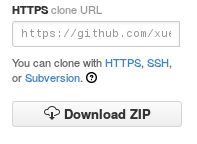
\includegraphics[width=.8\textwidth]{thuthesis-download.png}
          \end{figure}
        \end{column}
      \end{columns}
  \begin{itemize}
    \item 编译与安装
      \begin{itemize}
        \item 解压缩看文档 |README.md|
        \item Windows: 文件夹空白处按Shift+鼠标右键,点击“在此处打开命令行窗口”
        \item 模板文档类:|make cls| 编译 |thuthesis.dtx| $\Rightarrow$
          |thuthesis.cls|
        \item 论文示例:|make thesis| 编译 |thuthesis-example.tex| $\Rightarrow$
        |thuthesis-example.pdf|
        \item 用户手册:|make doc| 编译 |thuthesis.dtx| $\Rightarrow$
          |thuthesis.pdf|
        \item 更多用法可参考附带的 |Makefile|
      \end{itemize}
  \end{itemize}
\end{frame}

\begin{frame}[fragile]{模板选项}
\begin{description}
\item[degree] 指定学位类型(本科/硕士/博士/博后)
  \begin{lstlisting}[basicstyle=\ttfamily]
\documentclass[degree=bachelor]{thuthesis}
  \end{lstlisting}
\item[degree-type] 指定学位选项(专硕/学硕格式不同)
  \begin{lstlisting}[basicstyle=\ttfamily]
\documentclass[degree=master,degree-type=professional]{thuthesis}
  \end{lstlisting}
\item[fontset] 指定字体(推荐使用 |windows|,详见模板文档说明)
  \begin{lstlisting}[basicstyle=\ttfamily]
\documentclass[degree=doctor,fontset=windows]{thuthesis}
  \end{lstlisting}
\end{description}
\end{frame}

\begin{frame}[fragile]{封面}
  使用 |\thusetup| 命令指定论文各类选项:
  \begin{table}[h]
    \centering
\footnotesize
  \begin{tabular}{lll} \toprule
    命令作用 & 中文对应选项 & 英文对应选项 \\ \midrule
  论文标题 & |title| & |title*| \\
  作者姓名&  |author| &|author*|\\
  申请学位名称 & |degree-name|&|degree-name*|\\
  院系名称 & |department| & |department*|\\
  学科名称 & |discipline| & |discipline*|\\
  导师 & |supervisor| & |supervisor*|\\
  副导师 & |associate-supervisor| & |associate-supervisor*|\\
  联合导师 & |joint-supervisor| & |joint-supervisor*|\\
  日期 & \multicolumn{2}{c}{\texttt{date}}\\
  密级 & \multicolumn{2}{c}{\texttt{secret-year, secret-level}}\\
  语言(环境名称等) & \multicolumn{2}{c}{\texttt{language}} \\ 
  博后专用 & \multicolumn{2}{c}{\texttt{clc, udc, id, ...}} \\ \bottomrule
  \end{tabular}
  \end{table}
\end{frame}

\begin{frame}[fragile]{数学}
  \begin{itemize}
    \item 公式示例:\nolinkurl{data/chap01.tex}
    \item \ThuThesis{} 定义了常用的数学环境(需要手工引入 |amsthm| 宏包):
      \begin{table}[h]
        \centering
        \footnotesize
\begin{tabular}{*{7}{l}}\toprule
  axiom & theorem & definition & proposition & lemma & conjecture &\\
  公理 & 定理 & 定义 & 命题 & 引理 & 猜想 &\\\midrule
  proof & corollary & example & exercise & assumption & remark & problem \\
  证明 & 推论 & 例子& 练习 & 假设 & 注释 & 问题\\\bottomrule
\end{tabular}
      \end{table}
      \item \ThuThesis{} 使用 \pkg{unicode-math} 进行数学输入(\ref{frame:unicode-math} 页),注意与传统方式的区别
  \end{itemize}
\end{frame}

\begin{frame}[fragile]{参考文献}
  \begin{itemize}
    \item 使用 \BibTeX
      \begin{itemize}
        \item 使用文献管理软件导出 bib 文件
          \begin{itemize}
            \item Mendeley, NoteExpress
          \end{itemize}
        \item 使用 bibtex 生成参考文献列表
        \item 本科生文献翻译/阅读报告参考文献与正文独立
      \end{itemize}
    \item 模板支持两种引用方式:
      \begin{itemize}
        \item 顺序编码制,其中包含两种模式:
        \begin{itemize}
          \item 上标模式:如“在许多文献\textsuperscript{[12-13]}中……”
          \begin{lstlisting}[basicstyle=\ttfamily]
    \cite{key12, key13}
          \end{lstlisting}
        \item 正文模式:如“文献~[14] 证明了……”
          \begin{lstlisting}[basicstyle=\ttfamily]
    \inlinecite{key14}
          \end{lstlisting}
        \end{itemize}
        \item 著者-出版年制,包括两种引用模式(\cmd{citep}, \cmd{citet})
      \end{itemize}
    \end{itemize}
\end{frame}

% \begin{frame}{作图}
%   \begin{columns}[c]
%     \begin{column}{.5\textwidth}
%   \begin{itemize}
%   \item 矢量图 eps, ps, pdf
%     \begin{itemize}
%     \item \MP, pstricks, pgf $\ldots$
%     \item Xfig, Dia, \alert{Visio}, \alert{Inkscape} $\ldots$
%     \item Matlab / Excel 等保存为 pdf
%     \end{itemize}
%   \item 标量图 png, jpg, tiff $\ldots$
%     \begin{itemize}
%       \item 提高清晰度,避免发虚
%     \end{itemize}
%   \item 转化
%     \begin{itemize}
%     \item 虚拟打印机
%     \item ImageMagick
%     \item epstopdf
%     \item pdfcrop
%     \end{itemize}
%   \end{itemize}
%     \end{column}
%     \begin{column}{.4\textwidth}
% \begin{figure}[h]
%   \centering
% 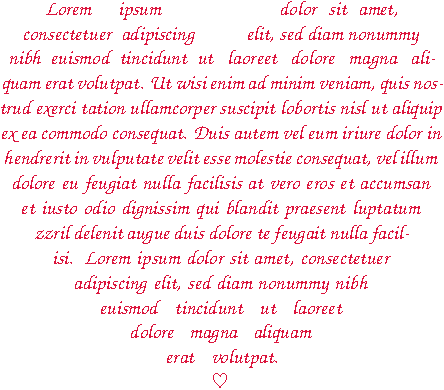
\includegraphics[height=.3\textheight]{shapepar.pdf}\\\vspace{1cm}
% 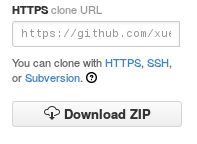
\includegraphics[height=.3\textheight]{thuthesis-download.png}
% \end{figure}
%     \end{column}
%   \end{columns}
% \end{frame}

\begin{frame}[fragile]{\ThuThesis 问题}
    \begin{itemize}
      \item 常见问题
        \begin{itemize}
          \item 参考文献列表出错、缺少字体、无法编译、格式不对……:先\textbf{更新到最新版本}试试
          \item 认真阅读文档 |thuthesis.pdf| 和使用示例 |thuthesis-example.pdf|
          \item 查看 FAQ \link{https://github.com/tuna/thuthesis/wiki/FAQ}
        \end{itemize}
      \item 主动提问
        \begin{itemize}
          \item GitHub Issues 提问:\link{https://github.com/tuna/thuthesis/issues}
          % \item \TeX @newsmth 查找或发文
          % \item \ThuThesis{} Google Group 发问 \link{http://groups.google.com/group/thuthesis}
        \end{itemize}
    \end{itemize}
\end{frame}



%%% vim: set sw=2 isk+=\: et tw=80 cc=+1 formatoptions+=mM:

% !TeX encoding = UTF-8
% !TeX program = xelatex
% !TeX root = latex-talk.tex

\section{总结}

\begin{frame}{常见 \LaTeX{} 问题}
  \begin{itemize}
    \item \alert{编译不通过} 缺少必要宏包,命令拼写错误,括号未配对等
    \item \alert{表格图片乱跑} \LaTeX{} 自身的浮动定位算法
    \item \alert{段落间距变大} \LaTeX{} 排版算法
    \item \alert{参考文献} 推荐使用 \BibTeX{} 或者 Bib\LaTeX{},也可以手写 \cmd{bibitem} \link{https://github.com/hushidong/biblatex-gb7714-2015}
  \end{itemize}
\end{frame}

\begin{frame}{系统学习}
  \begin{itemize}
      \item 包太雷 《\LaTeX{} Notes(第二版)》~(3小时)(lnotes2) \link{http://dralpha.altervista.org/zh/tech/lnotes2.pdf}
      \item Stefan Kottwitz 《LaTeX Cookbook》
      \item WikiBooks:英文 \link{https://en.wikibooks.org/wiki/LaTeX}、中文 \link{https://zh.wikibooks.org/wiki/LaTeX}
      \item 在线教程:ShareLaTeX、OverLeaf 都有帮助
      \item 经典文档
        \begin{itemize}
          \item 仔细阅读《一份不太简短的~\LaTeXe{} 介绍》(lshort-zh)~(1--2 天)
          \item 粗略阅读《\LaTeXe{} 插图指南》~(2--3 小时)
        \end{itemize}
      \item 仔细阅读《\ThuThesis{} 用户手册》~(20 分钟)
      \item 从~\ThuThesis{} 示例文档入手
  \end{itemize}
\end{frame}

\begin{frame}{扩展阅读}
  \begin{itemize}
    \item 一份其实很短的 \LaTeX 入门文档 (Liam Huang) \link{https://liam.page/2014/09/08/latex-introduction/}
    \item 网站推荐:
      \begin{itemize}
        \item http://www.latexstudio.net/
        \item http://www.chinatex.org/
      \end{itemize}
    \item 知乎 LaTeX 专栏: \url{http://zhuanlan.zhihu.com/LaTeX}
    \item \ThuThesis{}使用示例文档(模板自带)
    \item \LaTeX{}杂谈(刘海洋)
    \item 《\LaTeX{}入门》(刘海洋)
    \item 现代 LaTeX 入门讲座(曾祥东)\link{https://github.com/stone-zeng/latex-talk/releases/tag/2019-04-18}
    \item “黑科技”:在 \LaTeXe{} 中书写 Markdown 进行排版 \link{https://liam.page/2020/03/30/writing-manuscript-in-Markdown-and-typesetting-with-LaTeX/}
  \end{itemize}
\end{frame}


\begin{frame}{利用文档}
  \begin{itemize}
    \item 常用文档
      \begin{itemize}
        \item symbols: 符号大全
        \item Mathmode: 数学参考
        \item ctex, xeCJK: 中文支持
        \item texlive-zh: \TL 安装与使用
        \item 所用宏包文档
      \end{itemize}
    \item 工具
      \begin{itemize}
        \item tlmgr: \TL 管理器
        \item texdoc: \TeX{} 文档查看器\\
          例如:\texttt{texdoc lshort-zh}
        \item 在线文档 \TeX{}doc \link{http://texdoc.net/}
        \item TeX Studio 和 WinEdt 都支持在帮助里看文档
      \end{itemize}
  \end{itemize}
\end{frame}

\begin{frame}{一点人生的经验}
  \begin{itemize}
    \item 不要着急安装,先在 OverLeaf 上熟悉各类操作
    \item 不要过于相信网上的中文文档
      \begin{itemize}
        \item 简单鉴别方法: 排版的好看程度
      \end{itemize}
    \item 湿兄用U盘拷给你的的 C\TeX 套装一定是过时的,ThuThesis 八成是老版本的
    \item 如果你要处理中文
      \begin{itemize}
        \item 使用 XeLaTeX, 使用 XeLaTeX, 使用 XeLaTeX
        \item 忘记 CJK, 忘记 CJK, 忘记 CJK
        \item 使用 ctex 宏包(2.0以上版本)(跟 C\TeX 套装仅仅是名字像)
      \end{itemize}
    \item 写一点,编译一次,减小排错搜索空间
  \end{itemize}
\end{frame}

\begin{frame}[fragile]
  \frametitle{Git版本管理}
  \begin{itemize}
    \item 版本管理的必要性
      \begin{itemize}
        \item 远离「初稿,第二稿……终稿,终稿(打死也不改了)」命名
        \item 方便与他人协同合作
      \end{itemize}
    \item 基本用法
      \begin{itemize}
        \item 跟踪更改:|git init|、|git add|、|git commit|
        \item 撤销与回滚:|git reset|、|git revert|
        \item 分支与高级用法:|git branch|、|git checkout|、|git rebase|
        \item 远端仓库操作:|git pull|、|git push|、|git fetch|
        \item 推荐用 VS Code 等进行可视化操作
        \item 参考链接:\link{https://git-scm.com/book/en/v2}
          \link{https://www.liaoxuefeng.com/wiki/0013739516305929606dd18361248578c67b8067c8c017b000}
      \end{itemize}
    \item 在线 Git 服务
      \begin{itemize}
        \item GitHub \href{https://github.com}{\faGithub}
        \item 清华大学代码托管服务(基于 GitLab) \link{https://git.tsinghua.edu.cn}
      \end{itemize}
  \end{itemize}
  \end{frame}

% 寻求帮助
\begin{frame}{求助}
  \begin{columns}[c]
    \begin{column}{.45\textwidth}
      \begin{itemize}
        \item BBS
          \begin{itemize}
            \item 水木社区 TeX 版 \link{http://www.newsmth.net/nForum/board/TeX}
            \item CTEX 社区\link{http://bbs.ctex.org/}(从2018年底开始无限期关闭)
            \item 转移到 GitHub 的 CTEX 社区 \link{https://github.com/CTeX-org/forum}
          \end{itemize}
        \item UK FAQ \link{http://www.tex.ac.uk/cgi-bin/texfaq2html}
        \item TeX StackExchange \link{https://tex.stackexchange.com/}
        \item Google, Bing, etc.
          \begin{itemize}
            \item 使用\textbf{英语}搜索
          \end{itemize}
      \end{itemize}
    \end{column}
    \begin{column}{.45\textwidth}
      
\includegraphics[width=\textwidth]{TFZsuperellipse-crop.pdf}
    \end{column}
  \end{columns}
\end{frame}

\begin{frame}{你也可以帮助}
  \begin{itemize}
    \item 错误反馈、改进建议:GitHub Issues
    \item 出力维护:LaTeX 宏包编写、Git
    \item 科普、答疑 \hspace{2em}\sout{来当主讲人}
  \end{itemize}
\end{frame}

%%% vim: set ts=2 sts=2 sw=2 isk+=\: et tw=80 cc=+1 formatoptions+=mM:


\section*{附录}

\begin{frame}
  \begin{itemize}
    \item 本幻灯片:\url{https://github.com/tuna/thulib-latex-talk}
    \item 本幻灯片基于:
      \begin{itemize}
        \item \url{http://github.com/alick/fad-texlive-talk}
        \item \ThuThesis{}使用向导 v3.0
      \end{itemize}
    \item 许可证:CC BY-SA 4.0 Unported \cc\ccby\ccsa
  \end{itemize}
\end{frame}

\begin{frame}{扩展阅读}
  \begin{itemize}
    \item \LaTeX\ Tips:
      \url{https://alick.fedorapeople.org/fudcon-apac-2014/latex-tips.pdf} \\
      (例如:\LaTeX{} 中引号的正确输入姿势)
    \item Linux 用户:\url{https://github.com/alick/fad-texlive-talk}
    \item 网站推荐: http://www.latexstudio.net/
    \item 知乎专栏: http://zhuanlan.zhihu.com/LaTeX
    \item \ThuThesis{}使用向导 v3.0 (薛瑞尼)
    \item \LaTeX{}杂谈(刘海洋)
    \item 《\LaTeX{}入门》(刘海洋)
  \end{itemize}
\end{frame}

\begin{frame}
  \begin{center}
    {\Huge\calligra Thank you!}
  \end{center}
  \begin{figure}[htbp]
    \centering
    
\includegraphics[height=.2\textheight]{url.pdf}
  \end{figure}
\end{frame}

\end{document}

%%% vim: set ts=2 sts=2 sw=2 isk+=\: et tw=80 cc=+1 formatoptions+=mM:
